\documentclass[1p]{elsarticle_modified}
%\bibliographystyle{elsarticle-num}

%\usepackage[colorlinks]{hyperref}
%\usepackage{abbrmath_seonhwa} %\Abb, \Ascr, \Acal ,\Abf, \Afrak
\usepackage{amsfonts}
\usepackage{amssymb}
\usepackage{amsmath}
\usepackage{amsthm}
\usepackage{scalefnt}
\usepackage{amsbsy}
\usepackage{kotex}
\usepackage{caption}
\usepackage{subfig}
\usepackage{color}
\usepackage{graphicx}
\usepackage{xcolor} %% white, black, red, green, blue, cyan, magenta, yellow
\usepackage{float}
\usepackage{setspace}
\usepackage{hyperref}

\usepackage{tikz}
\usetikzlibrary{arrows}

\usepackage{multirow}
\usepackage{array} % fixed length table
\usepackage{hhline}

%%%%%%%%%%%%%%%%%%%%%
\makeatletter
\renewcommand*\env@matrix[1][\arraystretch]{%
	\edef\arraystretch{#1}%
	\hskip -\arraycolsep
	\let\@ifnextchar\new@ifnextchar
	\array{*\c@MaxMatrixCols c}}
\makeatother %https://tex.stackexchange.com/questions/14071/how-can-i-increase-the-line-spacing-in-a-matrix
%%%%%%%%%%%%%%%

\usepackage[normalem]{ulem}

\newcommand{\msout}[1]{\ifmmode\text{\sout{\ensuremath{#1}}}\else\sout{#1}\fi}
%SOURCE: \msout is \stkout macro in https://tex.stackexchange.com/questions/20609/strikeout-in-math-mode

\newcommand{\cancel}[1]{
	\ifmmode
	{\color{red}\msout{#1}}
	\else
	{\color{red}\sout{#1}}
	\fi
}

\newcommand{\add}[1]{
	{\color{blue}\uwave{#1}}
}

\newcommand{\replace}[2]{
	\ifmmode
	{\color{red}\msout{#1}}{\color{blue}\uwave{#2}}
	\else
	{\color{red}\sout{#1}}{\color{blue}\uwave{#2}}
	\fi
}

\newcommand{\Sol}{\mathcal{S}} %segment
\newcommand{\D}{D} %diagram
\newcommand{\A}{\mathcal{A}} %arc


%%%%%%%%%%%%%%%%%%%%%%%%%%%%%5 test

\def\sl{\operatorname{\textup{SL}}(2,\Cbb)}
\def\psl{\operatorname{\textup{PSL}}(2,\Cbb)}
\def\quan{\mkern 1mu \triangleright \mkern 1mu}

\theoremstyle{definition}
\newtheorem{thm}{Theorem}[section]
\newtheorem{prop}[thm]{Proposition}
\newtheorem{lem}[thm]{Lemma}
\newtheorem{ques}[thm]{Question}
\newtheorem{cor}[thm]{Corollary}
\newtheorem{defn}[thm]{Definition}
\newtheorem{exam}[thm]{Example}
\newtheorem{rmk}[thm]{Remark}
\newtheorem{alg}[thm]{Algorithm}

\newcommand{\I}{\sqrt{-1}}
\begin{document}

%\begin{frontmatter}
%
%\title{Boundary parabolic representations of knots up to 8 crossings}
%
%%% Group authors per affiliation:
%\author{Yunhi Cho} 
%\address{Department of Mathematics, University of Seoul, Seoul, Korea}
%\ead{yhcho@uos.ac.kr}
%
%
%\author{Seonhwa Kim} %\fnref{s_kim}}
%\address{Center for Geometry and Physics, Institute for Basic Science, Pohang, 37673, Korea}
%\ead{ryeona17@ibs.re.kr}
%
%\author{Hyuk Kim}
%\address{Department of Mathematical Sciences, Seoul National University, Seoul 08826, Korea}
%\ead{hyukkim@snu.ac.kr}
%
%\author{Seokbeom Yoon}
%\address{Department of Mathematical Sciences, Seoul National University, Seoul, 08826,  Korea}
%\ead{sbyoon15@snu.ac.kr}
%
%\begin{abstract}
%We find all boundary parabolic representation of knots up to 8 crossings.
%
%\end{abstract}
%\begin{keyword}
%    \MSC[2010] 57M25 
%\end{keyword}
%
%\end{frontmatter}

%\linenumbers
%\tableofcontents
%
\newcommand\colored[1]{\textcolor{white}{\rule[-0.35ex]{0.8em}{1.4ex}}\kern-0.8em\color{red} #1}%
%\newcommand\colored[1]{\textcolor{white}{ #1}\kern-2.17ex	\textcolor{white}{ #1}\kern-1.81ex	\textcolor{white}{ #1}\kern-2.15ex\color{red}#1	}

{\Large $\underline{12a_{0747}~(K12a_{0747})}$}

\setlength{\tabcolsep}{10pt}
\renewcommand{\arraystretch}{1.6}
\vspace{1cm}\begin{tabular}{m{100pt}>{\centering\arraybackslash}m{274pt}}
\multirow{5}{120pt}{
	\centering
	\includegraphics[width=112pt]{../../../GIT/diagram.site/Diagrams/png/1548_12a_0747.png}\\
\ \ \ A knot diagram\footnotemark}&
\allowdisplaybreaks
\textbf{Linearized knot diagam} \\
\cline{2-2}
 &
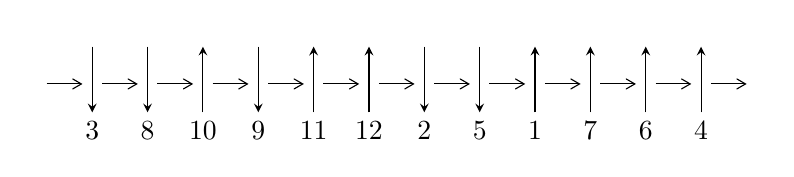
\begin{tikzpicture}[x=20pt, y=17pt]
	% nodes
	\node (C0) at (0, 0) {};
	\node (C1) at (1, 0) {};
	\node (C1U) at (1, +1) {};
	\node (C1D) at (1, -1) {3};

	\node (C2) at (2, 0) {};
	\node (C2U) at (2, +1) {};
	\node (C2D) at (2, -1) {8};

	\node (C3) at (3, 0) {};
	\node (C3U) at (3, +1) {};
	\node (C3D) at (3, -1) {10};

	\node (C4) at (4, 0) {};
	\node (C4U) at (4, +1) {};
	\node (C4D) at (4, -1) {9};

	\node (C5) at (5, 0) {};
	\node (C5U) at (5, +1) {};
	\node (C5D) at (5, -1) {11};

	\node (C6) at (6, 0) {};
	\node (C6U) at (6, +1) {};
	\node (C6D) at (6, -1) {12};

	\node (C7) at (7, 0) {};
	\node (C7U) at (7, +1) {};
	\node (C7D) at (7, -1) {2};

	\node (C8) at (8, 0) {};
	\node (C8U) at (8, +1) {};
	\node (C8D) at (8, -1) {5};

	\node (C9) at (9, 0) {};
	\node (C9U) at (9, +1) {};
	\node (C9D) at (9, -1) {1};

	\node (C10) at (10, 0) {};
	\node (C10U) at (10, +1) {};
	\node (C10D) at (10, -1) {7};

	\node (C11) at (11, 0) {};
	\node (C11U) at (11, +1) {};
	\node (C11D) at (11, -1) {6};

	\node (C12) at (12, 0) {};
	\node (C12U) at (12, +1) {};
	\node (C12D) at (12, -1) {4};
	\node (C13) at (13, 0) {};

	% arrows
	\draw[->,>={angle 60}]
	(C0) edge (C1) (C1) edge (C2) (C2) edge (C3) (C3) edge (C4) (C4) edge (C5) (C5) edge (C6) (C6) edge (C7) (C7) edge (C8) (C8) edge (C9) (C9) edge (C10) (C10) edge (C11) (C11) edge (C12) (C12) edge (C13) ;	\draw[->,>=stealth]
	(C1U) edge (C1D) (C2U) edge (C2D) (C3D) edge (C3U) (C4U) edge (C4D) (C5D) edge (C5U) (C6D) edge (C6U) (C7U) edge (C7D) (C8U) edge (C8D) (C9D) edge (C9U) (C10D) edge (C10U) (C11D) edge (C11U) (C12D) edge (C12U) ;
	\end{tikzpicture} \\
\hhline{~~} \\& 
\textbf{Solving Sequence} \\ \cline{2-2} 
 &
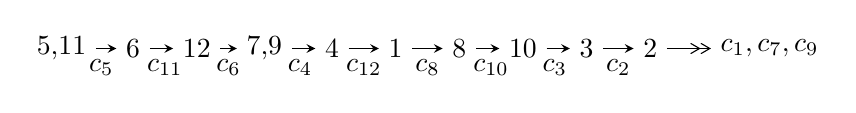
\begin{tikzpicture}[x=23pt, y=7pt]
	% node
	\node (A0) at (-1/8, 0) {5,11};
	\node (A1) at (1, 0) {6};
	\node (A2) at (2, 0) {12};
	\node (A3) at (49/16, 0) {7,9};
	\node (A4) at (33/8, 0) {4};
	\node (A5) at (41/8, 0) {1};
	\node (A6) at (49/8, 0) {8};
	\node (A7) at (57/8, 0) {10};
	\node (A8) at (65/8, 0) {3};
	\node (A9) at (73/8, 0) {2};
	\node (C1) at (1/2, -1) {$c_{5}$};
	\node (C2) at (3/2, -1) {$c_{11}$};
	\node (C3) at (5/2, -1) {$c_{6}$};
	\node (C4) at (29/8, -1) {$c_{4}$};
	\node (C5) at (37/8, -1) {$c_{12}$};
	\node (C6) at (45/8, -1) {$c_{8}$};
	\node (C7) at (53/8, -1) {$c_{10}$};
	\node (C8) at (61/8, -1) {$c_{3}$};
	\node (C9) at (69/8, -1) {$c_{2}$};
	\node (A10) at (11, 0) {$c_{1},c_{7},c_{9}$};

	% edge
	\draw[->,>=stealth]	
	(A0) edge (A1) (A1) edge (A2) (A2) edge (A3) (A3) edge (A4) (A4) edge (A5) (A5) edge (A6) (A6) edge (A7) (A7) edge (A8) (A8) edge (A9) ;
	\draw[->>,>={angle 60}]	
	(A9) edge (A10);
\end{tikzpicture} \\ 

\end{tabular} \\

\footnotetext{
The image of knot diagram is generated by the software ``\textbf{Draw programme}" developed by Andrew Bartholomew(\url{http://www.layer8.co.uk/maths/draw/index.htm\#Running-draw}), where we modified some parts for our purpose(\url{https://github.com/CATsTAILs/LinksPainter}).
}\phantom \\ \newline 
\centering \textbf{Ideals for irreducible components\footnotemark of $X_{\text{par}}$} 
 
\begin{align*}
I^u_{1}&=\langle 
2.65000\times10^{193} u^{128}+2.34665\times10^{193} u^{127}+\cdots+7.02232\times10^{193} b+2.48355\times10^{193},\\
\phantom{I^u_{1}}&\phantom{= \langle  }9.06725\times10^{193} u^{128}-2.07720\times10^{193} u^{127}+\cdots+7.02232\times10^{193} a-8.70594\times10^{193},\;u^{129}+u^{128}+\cdots-7 u-1\rangle \\
I^u_{2}&=\langle 
- u^{23}+11 u^{21}+\cdots+b-1,\;-3 u^{23}+32 u^{21}+\cdots+a-1,\;u^{24}-12 u^{22}+\cdots+2 u+1\rangle \\
\\
\end{align*}
\raggedright * 2 irreducible components of $\dim_{\mathbb{C}}=0$, with total 153 representations.\\
\footnotetext{All coefficients of polynomials are rational numbers. But the coefficients are sometimes approximated in decimal forms when there is not enough margin.}
\newpage
\renewcommand{\arraystretch}{1}
\centering \section*{I. $I^u_{1}= \langle 2.65\times10^{193} u^{128}+2.35\times10^{193} u^{127}+\cdots+7.02\times10^{193} b+2.48\times10^{193},\;9.07\times10^{193} u^{128}-2.08\times10^{193} u^{127}+\cdots+7.02\times10^{193} a-8.71\times10^{193},\;u^{129}+u^{128}+\cdots-7 u-1 \rangle$}
\flushleft \textbf{(i) Arc colorings}\\
\begin{tabular}{m{7pt} m{180pt} m{7pt} m{180pt} }
\flushright $a_{5}=$&$\begin{pmatrix}1\\0\end{pmatrix}$ \\
\flushright $a_{11}=$&$\begin{pmatrix}0\\u\end{pmatrix}$ \\
\flushright $a_{6}=$&$\begin{pmatrix}1\\- u^2\end{pmatrix}$ \\
\flushright $a_{12}=$&$\begin{pmatrix}u\\- u^3+u\end{pmatrix}$ \\
\flushright $a_{7}=$&$\begin{pmatrix}- u^2+1\\u^4-2 u^2\end{pmatrix}$ \\
\flushright $a_{9}=$&$\begin{pmatrix}-1.29120 u^{128}+0.295799 u^{127}+\cdots-1.43860 u+1.23975\\-0.377368 u^{128}-0.334169 u^{127}+\cdots+6.73997 u-0.353666\end{pmatrix}$ \\
\flushright $a_{4}=$&$\begin{pmatrix}0.871040 u^{128}+0.866622 u^{127}+\cdots-3.40452 u+4.53826\\-0.636934 u^{128}-0.772674 u^{127}+\cdots+13.3430 u+3.37451\end{pmatrix}$ \\
\flushright $a_{1}=$&$\begin{pmatrix}-1.41319 u^{128}-1.35974 u^{127}+\cdots+33.0349 u+4.89525\\-0.339303 u^{128}-0.689419 u^{127}+\cdots+12.1122 u+0.840007\end{pmatrix}$ \\
\flushright $a_{8}=$&$\begin{pmatrix}-1.66857 u^{128}-0.0383699 u^{127}+\cdots+5.30137 u+0.886086\\-0.377368 u^{128}-0.334169 u^{127}+\cdots+6.73997 u-0.353666\end{pmatrix}$ \\
\flushright $a_{10}=$&$\begin{pmatrix}- u^5+2 u^3- u\\u^7-3 u^5+2 u^3+u\end{pmatrix}$ \\
\flushright $a_{3}=$&$\begin{pmatrix}1.45033 u^{128}+0.399931 u^{127}+\cdots-5.09571 u+4.28260\\-1.10470 u^{128}-0.557067 u^{127}+\cdots+15.0987 u+3.65637\end{pmatrix}$ \\
\flushright $a_{2}=$&$\begin{pmatrix}0.478498 u^{128}+0.430788 u^{127}+\cdots+3.50990 u+2.48438\\0.0216946 u^{128}-0.0576587 u^{127}+\cdots+1.10851 u+1.82083\end{pmatrix}$\\&\end{tabular}
\flushleft \textbf{(ii) Obstruction class $= -1$}\\~\\
\flushleft \textbf{(iii) Cusp Shapes $= -3.51289 u^{128}-1.95504 u^{127}+\cdots+86.3712 u+22.6515$}\\~\\
\newpage\renewcommand{\arraystretch}{1}
\flushleft \textbf{(iv) u-Polynomials at the component}\newline \\
\begin{tabular}{m{50pt}|m{274pt}}
Crossings & \hspace{64pt}u-Polynomials at each crossing \\
\hline $$\begin{aligned}c_{1}\end{aligned}$$&$\begin{aligned}
&u^{129}+53 u^{128}+\cdots+241100 u+10201
\end{aligned}$\\
\hline $$\begin{aligned}c_{2},c_{7}\end{aligned}$$&$\begin{aligned}
&u^{129}+u^{128}+\cdots-268 u-101
\end{aligned}$\\
\hline $$\begin{aligned}c_{3}\end{aligned}$$&$\begin{aligned}
&u^{129}-6 u^{127}+\cdots-141 u-9
\end{aligned}$\\
\hline $$\begin{aligned}c_{4},c_{8}\end{aligned}$$&$\begin{aligned}
&u^{129}+2 u^{128}+\cdots-21685 u-15853
\end{aligned}$\\
\hline $$\begin{aligned}c_{5},c_{6},c_{11}\end{aligned}$$&$\begin{aligned}
&u^{129}+u^{128}+\cdots-7 u-1
\end{aligned}$\\
\hline $$\begin{aligned}c_{9}\end{aligned}$$&$\begin{aligned}
&u^{129}-7 u^{128}+\cdots+31027 u+4567
\end{aligned}$\\
\hline $$\begin{aligned}c_{10}\end{aligned}$$&$\begin{aligned}
&u^{129}-3 u^{128}+\cdots+22569 u+1491
\end{aligned}$\\
\hline $$\begin{aligned}c_{12}\end{aligned}$$&$\begin{aligned}
&u^{129}+11 u^{128}+\cdots-170 u+29
\end{aligned}$\\
\hline
\end{tabular}\\~\\
\newpage\renewcommand{\arraystretch}{1}
\flushleft \textbf{(v) Riley Polynomials at the component}\newline \\
\begin{tabular}{m{50pt}|m{274pt}}
Crossings & \hspace{64pt}Riley Polynomials at each crossing \\
\hline $$\begin{aligned}c_{1}\end{aligned}$$&$\begin{aligned}
&y^{129}+59 y^{128}+\cdots+6188411064 y-104060401
\end{aligned}$\\
\hline $$\begin{aligned}c_{2},c_{7}\end{aligned}$$&$\begin{aligned}
&y^{129}-53 y^{128}+\cdots+241100 y-10201
\end{aligned}$\\
\hline $$\begin{aligned}c_{3}\end{aligned}$$&$\begin{aligned}
&y^{129}-12 y^{128}+\cdots+369 y-81
\end{aligned}$\\
\hline $$\begin{aligned}c_{4},c_{8}\end{aligned}$$&$\begin{aligned}
&y^{129}+92 y^{128}+\cdots-5214202691 y-251317609
\end{aligned}$\\
\hline $$\begin{aligned}c_{5},c_{6},c_{11}\end{aligned}$$&$\begin{aligned}
&y^{129}-117 y^{128}+\cdots-19 y-1
\end{aligned}$\\
\hline $$\begin{aligned}c_{9}\end{aligned}$$&$\begin{aligned}
&y^{129}-37 y^{128}+\cdots+3096724221 y-20857489
\end{aligned}$\\
\hline $$\begin{aligned}c_{10}\end{aligned}$$&$\begin{aligned}
&y^{129}+15 y^{128}+\cdots+34052817 y-2223081
\end{aligned}$\\
\hline $$\begin{aligned}c_{12}\end{aligned}$$&$\begin{aligned}
&y^{129}-17 y^{128}+\cdots+61496 y-841
\end{aligned}$\\
\hline
\end{tabular}\\~\\
\newpage\flushleft \textbf{(vi) Complex Volumes and Cusp Shapes}
$$\begin{array}{c|c|c}  
\text{Solutions to }I^u_{1}& \I (\text{vol} + \sqrt{-1}CS) & \text{Cusp shape}\\
 \hline 
\begin{aligned}
u &= \phantom{-}0.051970 + 0.993015 I \\
a &= \phantom{-}0.0380113 - 0.0039953 I \\
b &= \phantom{-}0.098904 + 0.986419 I\end{aligned}
 & -1.64979 - 2.02859 I & \phantom{-0.000000 } 0 \\ \hline\begin{aligned}
u &= \phantom{-}0.051970 - 0.993015 I \\
a &= \phantom{-}0.0380113 + 0.0039953 I \\
b &= \phantom{-}0.098904 - 0.986419 I\end{aligned}
 & -1.64979 + 2.02859 I & \phantom{-0.000000 } 0 \\ \hline\begin{aligned}
u &= \phantom{-}0.837971 + 0.567834 I \\
a &= \phantom{-}0.477899 + 0.591226 I \\
b &= -0.496140 - 1.298570 I\end{aligned}
 & \phantom{-}3.24310 - 9.68057 I & \phantom{-0.000000 } 0 \\ \hline\begin{aligned}
u &= \phantom{-}0.837971 - 0.567834 I \\
a &= \phantom{-}0.477899 - 0.591226 I \\
b &= -0.496140 + 1.298570 I\end{aligned}
 & \phantom{-}3.24310 + 9.68057 I & \phantom{-0.000000 } 0 \\ \hline\begin{aligned}
u &= \phantom{-}1.025480 + 0.237033 I \\
a &= -0.162210 + 1.010220 I \\
b &= -0.520771 - 1.046700 I\end{aligned}
 & -0.73696 - 2.43278 I & \phantom{-0.000000 } 0 \\ \hline\begin{aligned}
u &= \phantom{-}1.025480 - 0.237033 I \\
a &= -0.162210 - 1.010220 I \\
b &= -0.520771 + 1.046700 I\end{aligned}
 & -0.73696 + 2.43278 I & \phantom{-0.000000 } 0 \\ \hline\begin{aligned}
u &= -0.509412 + 0.784048 I \\
a &= \phantom{-}0.783191 - 0.998753 I \\
b &= \phantom{-}0.321116 + 0.820314 I\end{aligned}
 & -1.33885 - 5.56038 I & \phantom{-0.000000 } 0 \\ \hline\begin{aligned}
u &= -0.509412 - 0.784048 I \\
a &= \phantom{-}0.783191 + 0.998753 I \\
b &= \phantom{-}0.321116 - 0.820314 I\end{aligned}
 & -1.33885 + 5.56038 I & \phantom{-0.000000 } 0 \\ \hline\begin{aligned}
u &= \phantom{-}1.053430 + 0.175522 I \\
a &= -0.353167 - 0.153552 I \\
b &= \phantom{-}0.059796 - 1.051140 I\end{aligned}
 & \phantom{-}3.69303 - 2.14193 I & \phantom{-0.000000 } 0 \\ \hline\begin{aligned}
u &= \phantom{-}1.053430 - 0.175522 I \\
a &= -0.353167 + 0.153552 I \\
b &= \phantom{-}0.059796 + 1.051140 I\end{aligned}
 & \phantom{-}3.69303 + 2.14193 I & \phantom{-0.000000 } 0\\
 \hline 
 \end{array}$$\newpage$$\begin{array}{c|c|c}  
\text{Solutions to }I^u_{1}& \I (\text{vol} + \sqrt{-1}CS) & \text{Cusp shape}\\
 \hline 
\begin{aligned}
u &= \phantom{-}0.732149 + 0.526761 I \\
a &= -0.772088 - 1.096370 I \\
b &= -0.420090 + 0.967338 I\end{aligned}
 & \phantom{-}0.11355 + 2.39050 I & \phantom{-0.000000 } 0 \\ \hline\begin{aligned}
u &= \phantom{-}0.732149 - 0.526761 I \\
a &= -0.772088 + 1.096370 I \\
b &= -0.420090 - 0.967338 I\end{aligned}
 & \phantom{-}0.11355 - 2.39050 I & \phantom{-0.000000 } 0 \\ \hline\begin{aligned}
u &= -0.732811 + 0.525422 I \\
a &= -0.659964 + 0.737980 I \\
b &= \phantom{-}0.398953 - 1.261590 I\end{aligned}
 & \phantom{-}4.91057 + 4.11692 I & \phantom{-0.000000 } 0 \\ \hline\begin{aligned}
u &= -0.732811 - 0.525422 I \\
a &= -0.659964 - 0.737980 I \\
b &= \phantom{-}0.398953 + 1.261590 I\end{aligned}
 & \phantom{-}4.91057 - 4.11692 I & \phantom{-0.000000 } 0 \\ \hline\begin{aligned}
u &= \phantom{-}0.309866 + 0.831253 I \\
a &= \phantom{-}1.243500 + 0.568619 I \\
b &= \phantom{-}0.58944 - 1.35556 I\end{aligned}
 & \phantom{-}1.5905 + 14.5341 I & \phantom{-0.000000 } 0 \\ \hline\begin{aligned}
u &= \phantom{-}0.309866 - 0.831253 I \\
a &= \phantom{-}1.243500 - 0.568619 I \\
b &= \phantom{-}0.58944 + 1.35556 I\end{aligned}
 & \phantom{-}1.5905 - 14.5341 I & \phantom{-0.000000 } 0 \\ \hline\begin{aligned}
u &= \phantom{-}1.113440 + 0.093009 I \\
a &= -0.227047 + 0.880009 I \\
b &= \phantom{-}0.804580 - 0.313020 I\end{aligned}
 & \phantom{-}1.64515 - 0.14115 I & \phantom{-0.000000 } 0 \\ \hline\begin{aligned}
u &= \phantom{-}1.113440 - 0.093009 I \\
a &= -0.227047 - 0.880009 I \\
b &= \phantom{-}0.804580 + 0.313020 I\end{aligned}
 & \phantom{-}1.64515 + 0.14115 I & \phantom{-0.000000 } 0 \\ \hline\begin{aligned}
u &= -1.124460 + 0.151681 I \\
a &= \phantom{-}0.682863 + 0.052497 I \\
b &= -0.586833 + 1.072260 I\end{aligned}
 & \phantom{-}4.88050 + 2.27576 I & \phantom{-0.000000 } 0 \\ \hline\begin{aligned}
u &= -1.124460 - 0.151681 I \\
a &= \phantom{-}0.682863 - 0.052497 I \\
b &= -0.586833 - 1.072260 I\end{aligned}
 & \phantom{-}4.88050 - 2.27576 I & \phantom{-0.000000 } 0\\
 \hline 
 \end{array}$$\newpage$$\begin{array}{c|c|c}  
\text{Solutions to }I^u_{1}& \I (\text{vol} + \sqrt{-1}CS) & \text{Cusp shape}\\
 \hline 
\begin{aligned}
u &= -0.321690 + 0.772157 I \\
a &= -1.206270 + 0.699130 I \\
b &= -0.50767 - 1.34684 I\end{aligned}
 & \phantom{-}3.55448 - 8.60382 I & \phantom{-0.000000 } 0 \\ \hline\begin{aligned}
u &= -0.321690 - 0.772157 I \\
a &= -1.206270 - 0.699130 I \\
b &= -0.50767 + 1.34684 I\end{aligned}
 & \phantom{-}3.55448 + 8.60382 I & \phantom{-0.000000 } 0 \\ \hline\begin{aligned}
u &= -0.242794 + 0.796642 I \\
a &= \phantom{-}0.428709 - 0.858731 I \\
b &= \phantom{-}0.107481 + 0.811941 I\end{aligned}
 & -2.10827 + 0.88291 I & \phantom{-0.000000 } 0 \\ \hline\begin{aligned}
u &= -0.242794 - 0.796642 I \\
a &= \phantom{-}0.428709 + 0.858731 I \\
b &= \phantom{-}0.107481 - 0.811941 I\end{aligned}
 & -2.10827 - 0.88291 I & \phantom{-0.000000 } 0 \\ \hline\begin{aligned}
u &= \phantom{-}0.228527 + 0.798986 I \\
a &= \phantom{-}0.188913 - 0.123671 I \\
b &= \phantom{-}0.409325 + 0.670158 I\end{aligned}
 & -1.67570 + 2.20914 I & \phantom{-0.000000 } 0 \\ \hline\begin{aligned}
u &= \phantom{-}0.228527 - 0.798986 I \\
a &= \phantom{-}0.188913 + 0.123671 I \\
b &= \phantom{-}0.409325 - 0.670158 I\end{aligned}
 & -1.67570 - 2.20914 I & \phantom{-0.000000 } 0 \\ \hline\begin{aligned}
u &= -0.826691 + 0.041202 I \\
a &= -0.06131 + 1.44905 I \\
b &= -0.712028 - 0.154552 I\end{aligned}
 & -0.54483 + 4.69995 I & \phantom{-0.000000 } 0 \\ \hline\begin{aligned}
u &= -0.826691 - 0.041202 I \\
a &= -0.06131 - 1.44905 I \\
b &= -0.712028 + 0.154552 I\end{aligned}
 & -0.54483 - 4.69995 I & \phantom{-0.000000 } 0 \\ \hline\begin{aligned}
u &= -1.143590 + 0.286522 I \\
a &= -0.365462 + 0.654972 I \\
b &= -0.781152 - 0.421442 I\end{aligned}
 & -2.66439 - 2.38185 I & \phantom{-0.000000 } 0 \\ \hline\begin{aligned}
u &= -1.143590 - 0.286522 I \\
a &= -0.365462 - 0.654972 I \\
b &= -0.781152 + 0.421442 I\end{aligned}
 & -2.66439 + 2.38185 I & \phantom{-0.000000 } 0\\
 \hline 
 \end{array}$$\newpage$$\begin{array}{c|c|c}  
\text{Solutions to }I^u_{1}& \I (\text{vol} + \sqrt{-1}CS) & \text{Cusp shape}\\
 \hline 
\begin{aligned}
u &= -1.209850 + 0.231073 I \\
a &= -0.006204 - 1.069620 I \\
b &= \phantom{-}0.580455 + 0.696591 I\end{aligned}
 & \phantom{-}2.68604 - 4.47896 I & \phantom{-0.000000 } 0 \\ \hline\begin{aligned}
u &= -1.209850 - 0.231073 I \\
a &= -0.006204 + 1.069620 I \\
b &= \phantom{-}0.580455 - 0.696591 I\end{aligned}
 & \phantom{-}2.68604 + 4.47896 I & \phantom{-0.000000 } 0 \\ \hline\begin{aligned}
u &= -0.093034 + 0.753912 I \\
a &= \phantom{-}0.692986 - 0.562528 I \\
b &= \phantom{-}0.787377 - 0.323100 I\end{aligned}
 & -5.84209 - 1.43644 I & -6.45657 + 1.49198 I \\ \hline\begin{aligned}
u &= -0.093034 - 0.753912 I \\
a &= \phantom{-}0.692986 + 0.562528 I \\
b &= \phantom{-}0.787377 + 0.323100 I\end{aligned}
 & -5.84209 + 1.43644 I & -6.45657 - 1.49198 I \\ \hline\begin{aligned}
u &= -0.241534 + 0.709885 I \\
a &= \phantom{-}0.876196 - 0.390382 I \\
b &= \phantom{-}1.218590 - 0.100809 I\end{aligned}
 & -2.40215 - 8.26114 I & -0.87236 + 9.14716 I \\ \hline\begin{aligned}
u &= -0.241534 - 0.709885 I \\
a &= \phantom{-}0.876196 + 0.390382 I \\
b &= \phantom{-}1.218590 + 0.100809 I\end{aligned}
 & -2.40215 + 8.26114 I & -0.87236 - 9.14716 I \\ \hline\begin{aligned}
u &= \phantom{-}0.399018 + 0.623768 I \\
a &= -0.874191 - 0.740196 I \\
b &= -0.243009 + 0.990794 I\end{aligned}
 & \phantom{-}0.71421 + 1.90496 I & \phantom{-}2.00000 - 4.65501 I \\ \hline\begin{aligned}
u &= \phantom{-}0.399018 - 0.623768 I \\
a &= -0.874191 + 0.740196 I \\
b &= -0.243009 - 0.990794 I\end{aligned}
 & \phantom{-}0.71421 - 1.90496 I & \phantom{-}2.00000 + 4.65501 I \\ \hline\begin{aligned}
u &= \phantom{-}0.181659 + 0.706610 I \\
a &= \phantom{-}1.65849 + 0.89371 I \\
b &= \phantom{-}0.450536 - 1.148240 I\end{aligned}
 & -3.24329 + 6.01733 I & -2.16925 - 7.40566 I \\ \hline\begin{aligned}
u &= \phantom{-}0.181659 - 0.706610 I \\
a &= \phantom{-}1.65849 - 0.89371 I \\
b &= \phantom{-}0.450536 + 1.148240 I\end{aligned}
 & -3.24329 - 6.01733 I & -2.16925 + 7.40566 I\\
 \hline 
 \end{array}$$\newpage$$\begin{array}{c|c|c}  
\text{Solutions to }I^u_{1}& \I (\text{vol} + \sqrt{-1}CS) & \text{Cusp shape}\\
 \hline 
\begin{aligned}
u &= \phantom{-}0.185623 + 0.701396 I \\
a &= \phantom{-}1.86550 - 0.58997 I \\
b &= \phantom{-}0.165893 - 1.071950 I\end{aligned}
 & \phantom{-}1.21465 + 5.56964 I & \phantom{-}5.61858 - 8.19173 I \\ \hline\begin{aligned}
u &= \phantom{-}0.185623 - 0.701396 I \\
a &= \phantom{-}1.86550 + 0.58997 I \\
b &= \phantom{-}0.165893 + 1.071950 I\end{aligned}
 & \phantom{-}1.21465 - 5.56964 I & \phantom{-}5.61858 + 8.19173 I \\ \hline\begin{aligned}
u &= \phantom{-}1.144770 + 0.562586 I \\
a &= -0.505538 - 0.793395 I \\
b &= -0.235197 + 1.068220 I\end{aligned}
 & \phantom{-}1.70104 + 7.45697 I & \phantom{-0.000000 } 0 \\ \hline\begin{aligned}
u &= \phantom{-}1.144770 - 0.562586 I \\
a &= -0.505538 + 0.793395 I \\
b &= -0.235197 - 1.068220 I\end{aligned}
 & \phantom{-}1.70104 - 7.45697 I & \phantom{-0.000000 } 0 \\ \hline\begin{aligned}
u &= \phantom{-}0.295679 + 0.651657 I \\
a &= -1.48088 - 0.06488 I \\
b &= -0.57041 + 1.38485 I\end{aligned}
 & \phantom{-}2.72621 + 0.81441 I & \phantom{-}6.95955 - 1.10717 I \\ \hline\begin{aligned}
u &= \phantom{-}0.295679 - 0.651657 I \\
a &= -1.48088 + 0.06488 I \\
b &= -0.57041 - 1.38485 I\end{aligned}
 & \phantom{-}2.72621 - 0.81441 I & \phantom{-}6.95955 + 1.10717 I \\ \hline\begin{aligned}
u &= -0.706698 + 0.009775 I \\
a &= -0.04253 + 1.54520 I \\
b &= -0.661366 - 0.064571 I\end{aligned}
 & -0.54610 + 4.70193 I & \phantom{-}0.76536 - 4.65762 I \\ \hline\begin{aligned}
u &= -0.706698 - 0.009775 I \\
a &= -0.04253 - 1.54520 I \\
b &= -0.661366 + 0.064571 I\end{aligned}
 & -0.54610 - 4.70193 I & \phantom{-}0.76536 + 4.65762 I \\ \hline\begin{aligned}
u &= -0.188008 + 0.672153 I \\
a &= \phantom{-}1.66160 + 0.13653 I \\
b &= \phantom{-}0.76344 + 1.31899 I\end{aligned}
 & \phantom{-}2.30526 - 5.39595 I & \phantom{-}4.61743 + 7.91302 I \\ \hline\begin{aligned}
u &= -0.188008 - 0.672153 I \\
a &= \phantom{-}1.66160 - 0.13653 I \\
b &= \phantom{-}0.76344 - 1.31899 I\end{aligned}
 & \phantom{-}2.30526 + 5.39595 I & \phantom{-}4.61743 - 7.91302 I\\
 \hline 
 \end{array}$$\newpage$$\begin{array}{c|c|c}  
\text{Solutions to }I^u_{1}& \I (\text{vol} + \sqrt{-1}CS) & \text{Cusp shape}\\
 \hline 
\begin{aligned}
u &= \phantom{-}1.31835\phantom{ +0.000000I} \\
a &= -0.682453\phantom{ +0.000000I} \\
b &= \phantom{-}0.815064\phantom{ +0.000000I}\end{aligned}
 & \phantom{-}3.05905\phantom{ +0.000000I} & \phantom{-0.000000 } 0 \\ \hline\begin{aligned}
u &= \phantom{-}0.191951 + 0.647839 I \\
a &= -0.794070 - 0.291142 I \\
b &= -1.083280 + 0.054850 I\end{aligned}
 & -0.79396 + 3.05732 I & \phantom{-}0.59352 - 5.00231 I \\ \hline\begin{aligned}
u &= \phantom{-}0.191951 - 0.647839 I \\
a &= -0.794070 + 0.291142 I \\
b &= -1.083280 - 0.054850 I\end{aligned}
 & -0.79396 - 3.05732 I & \phantom{-}0.59352 + 5.00231 I \\ \hline\begin{aligned}
u &= \phantom{-}1.331690 + 0.153637 I \\
a &= -0.90494 - 2.57744 I \\
b &= -0.657321 + 1.119200 I\end{aligned}
 & \phantom{-}5.10259 + 3.32211 I & \phantom{-0.000000 } 0 \\ \hline\begin{aligned}
u &= \phantom{-}1.331690 - 0.153637 I \\
a &= -0.90494 + 2.57744 I \\
b &= -0.657321 - 1.119200 I\end{aligned}
 & \phantom{-}5.10259 - 3.32211 I & \phantom{-0.000000 } 0 \\ \hline\begin{aligned}
u &= -1.249700 + 0.492475 I \\
a &= \phantom{-}0.398034 - 0.700256 I \\
b &= \phantom{-}0.049981 + 0.968730 I\end{aligned}
 & \phantom{-}2.35727 - 3.21528 I & \phantom{-0.000000 } 0 \\ \hline\begin{aligned}
u &= -1.249700 - 0.492475 I \\
a &= \phantom{-}0.398034 + 0.700256 I \\
b &= \phantom{-}0.049981 - 0.968730 I\end{aligned}
 & \phantom{-}2.35727 + 3.21528 I & \phantom{-0.000000 } 0 \\ \hline\begin{aligned}
u &= -1.343850 + 0.142360 I \\
a &= -1.45232 + 3.03674 I \\
b &= \phantom{-}0.028054 - 1.023450 I\end{aligned}
 & \phantom{-}3.74547 + 2.60657 I & \phantom{-0.000000 } 0 \\ \hline\begin{aligned}
u &= -1.343850 - 0.142360 I \\
a &= -1.45232 - 3.03674 I \\
b &= \phantom{-}0.028054 + 1.023450 I\end{aligned}
 & \phantom{-}3.74547 - 2.60657 I & \phantom{-0.000000 } 0 \\ \hline\begin{aligned}
u &= \phantom{-}1.314300 + 0.320206 I \\
a &= \phantom{-}0.404246 - 0.664630 I \\
b &= -0.758072 - 0.266299 I\end{aligned}
 & -1.43950 + 5.31733 I & \phantom{-0.000000 } 0\\
 \hline 
 \end{array}$$\newpage$$\begin{array}{c|c|c}  
\text{Solutions to }I^u_{1}& \I (\text{vol} + \sqrt{-1}CS) & \text{Cusp shape}\\
 \hline 
\begin{aligned}
u &= \phantom{-}1.314300 - 0.320206 I \\
a &= \phantom{-}0.404246 + 0.664630 I \\
b &= -0.758072 + 0.266299 I\end{aligned}
 & -1.43950 - 5.31733 I & \phantom{-0.000000 } 0 \\ \hline\begin{aligned}
u &= -1.347630 + 0.125395 I \\
a &= \phantom{-}0.42870 + 2.55795 I \\
b &= \phantom{-}0.229918 - 1.343880 I\end{aligned}
 & \phantom{-}8.43775 + 2.00284 I & \phantom{-0.000000 } 0 \\ \hline\begin{aligned}
u &= -1.347630 - 0.125395 I \\
a &= \phantom{-}0.42870 - 2.55795 I \\
b &= \phantom{-}0.229918 + 1.343880 I\end{aligned}
 & \phantom{-}8.43775 - 2.00284 I & \phantom{-0.000000 } 0 \\ \hline\begin{aligned}
u &= -1.360310 + 0.084915 I \\
a &= \phantom{-}0.819748 - 0.021975 I \\
b &= \phantom{-}0.145792 - 0.333836 I\end{aligned}
 & \phantom{-}6.59527 - 1.16256 I & \phantom{-0.000000 } 0 \\ \hline\begin{aligned}
u &= -1.360310 - 0.084915 I \\
a &= \phantom{-}0.819748 + 0.021975 I \\
b &= \phantom{-}0.145792 + 0.333836 I\end{aligned}
 & \phantom{-}6.59527 + 1.16256 I & \phantom{-0.000000 } 0 \\ \hline\begin{aligned}
u &= -1.354540 + 0.171932 I \\
a &= \phantom{-}0.673046 + 0.107343 I \\
b &= -1.081530 + 0.769859 I\end{aligned}
 & \phantom{-}5.44556 - 0.86088 I & \phantom{-0.000000 } 0 \\ \hline\begin{aligned}
u &= -1.354540 - 0.171932 I \\
a &= \phantom{-}0.673046 - 0.107343 I \\
b &= -1.081530 - 0.769859 I\end{aligned}
 & \phantom{-}5.44556 + 0.86088 I & \phantom{-0.000000 } 0 \\ \hline\begin{aligned}
u &= \phantom{-}1.368210 + 0.143378 I \\
a &= -1.18519 - 2.16747 I \\
b &= \phantom{-}0.50495 + 1.76954 I\end{aligned}
 & \phantom{-}9.08592 - 1.40627 I & \phantom{-0.000000 } 0 \\ \hline\begin{aligned}
u &= \phantom{-}1.368210 - 0.143378 I \\
a &= -1.18519 + 2.16747 I \\
b &= \phantom{-}0.50495 - 1.76954 I\end{aligned}
 & \phantom{-}9.08592 + 1.40627 I & \phantom{-0.000000 } 0 \\ \hline\begin{aligned}
u &= -0.274204 + 0.559986 I \\
a &= -2.20159 + 0.37589 I \\
b &= \phantom{-}0.023992 - 1.078520 I\end{aligned}
 & \phantom{-}3.75901 + 0.50385 I & \phantom{-}8.87364 + 0.38982 I\\
 \hline 
 \end{array}$$\newpage$$\begin{array}{c|c|c}  
\text{Solutions to }I^u_{1}& \I (\text{vol} + \sqrt{-1}CS) & \text{Cusp shape}\\
 \hline 
\begin{aligned}
u &= -0.274204 - 0.559986 I \\
a &= -2.20159 - 0.37589 I \\
b &= \phantom{-}0.023992 + 1.078520 I\end{aligned}
 & \phantom{-}3.75901 - 0.50385 I & \phantom{-}8.87364 - 0.38982 I \\ \hline\begin{aligned}
u &= \phantom{-}1.372760 + 0.178307 I \\
a &= -0.835735 + 0.072782 I \\
b &= -0.376647 - 0.507264 I\end{aligned}
 & \phantom{-}4.34556 + 6.41095 I & \phantom{-0.000000 } 0 \\ \hline\begin{aligned}
u &= \phantom{-}1.372760 - 0.178307 I \\
a &= -0.835735 - 0.072782 I \\
b &= -0.376647 + 0.507264 I\end{aligned}
 & \phantom{-}4.34556 - 6.41095 I & \phantom{-0.000000 } 0 \\ \hline\begin{aligned}
u &= -0.396188 + 0.471004 I \\
a &= -0.203653 - 0.409084 I \\
b &= -0.485022 + 0.338354 I\end{aligned}
 & -1.47214 + 1.29483 I & -2.21582 - 0.22695 I \\ \hline\begin{aligned}
u &= -0.396188 - 0.471004 I \\
a &= -0.203653 + 0.409084 I \\
b &= -0.485022 - 0.338354 I\end{aligned}
 & -1.47214 - 1.29483 I & -2.21582 + 0.22695 I \\ \hline\begin{aligned}
u &= \phantom{-}1.370430 + 0.219938 I \\
a &= -0.244267 - 0.140422 I \\
b &= \phantom{-}0.697716 + 0.149710 I\end{aligned}
 & \phantom{-}3.72148 + 1.22839 I & \phantom{-0.000000 } 0 \\ \hline\begin{aligned}
u &= \phantom{-}1.370430 - 0.219938 I \\
a &= -0.244267 + 0.140422 I \\
b &= \phantom{-}0.697716 - 0.149710 I\end{aligned}
 & \phantom{-}3.72148 - 1.22839 I & \phantom{-0.000000 } 0 \\ \hline\begin{aligned}
u &= -1.373840 + 0.254943 I \\
a &= -0.586959 - 0.911580 I \\
b &= \phantom{-}1.272080 + 0.161262 I\end{aligned}
 & \phantom{-}4.18347 - 6.34498 I & \phantom{-0.000000 } 0 \\ \hline\begin{aligned}
u &= -1.373840 - 0.254943 I \\
a &= -0.586959 + 0.911580 I \\
b &= \phantom{-}1.272080 - 0.161262 I\end{aligned}
 & \phantom{-}4.18347 + 6.34498 I & \phantom{-0.000000 } 0 \\ \hline\begin{aligned}
u &= \phantom{-}1.384740 + 0.189290 I \\
a &= \phantom{-}0.36841 + 3.00144 I \\
b &= \phantom{-}0.064495 - 1.369760 I\end{aligned}
 & \phantom{-}9.53240 + 5.59842 I & \phantom{-0.000000 } 0\\
 \hline 
 \end{array}$$\newpage$$\begin{array}{c|c|c}  
\text{Solutions to }I^u_{1}& \I (\text{vol} + \sqrt{-1}CS) & \text{Cusp shape}\\
 \hline 
\begin{aligned}
u &= \phantom{-}1.384740 - 0.189290 I \\
a &= \phantom{-}0.36841 - 3.00144 I \\
b &= \phantom{-}0.064495 + 1.369760 I\end{aligned}
 & \phantom{-}9.53240 - 5.59842 I & \phantom{-0.000000 } 0 \\ \hline\begin{aligned}
u &= -1.370920 + 0.280112 I \\
a &= -1.31613 + 2.52051 I \\
b &= -0.398798 - 1.227510 I\end{aligned}
 & \phantom{-}1.68222 - 9.58894 I & \phantom{-0.000000 } 0 \\ \hline\begin{aligned}
u &= -1.370920 - 0.280112 I \\
a &= -1.31613 - 2.52051 I \\
b &= -0.398798 + 1.227510 I\end{aligned}
 & \phantom{-}1.68222 + 9.58894 I & \phantom{-0.000000 } 0 \\ \hline\begin{aligned}
u &= -1.372400 + 0.281414 I \\
a &= -1.85494 + 1.11740 I \\
b &= -0.264635 - 1.089620 I\end{aligned}
 & \phantom{-}6.15824 - 9.13709 I & \phantom{-0.000000 } 0 \\ \hline\begin{aligned}
u &= -1.372400 - 0.281414 I \\
a &= -1.85494 - 1.11740 I \\
b &= -0.264635 + 1.089620 I\end{aligned}
 & \phantom{-}6.15824 + 9.13709 I & \phantom{-0.000000 } 0 \\ \hline\begin{aligned}
u &= \phantom{-}1.375060 + 0.269737 I \\
a &= -0.95851 - 2.06127 I \\
b &= -0.88247 + 1.43103 I\end{aligned}
 & \phantom{-}7.27555 + 8.82792 I & \phantom{-0.000000 } 0 \\ \hline\begin{aligned}
u &= \phantom{-}1.375060 - 0.269737 I \\
a &= -0.95851 + 2.06127 I \\
b &= -0.88247 - 1.43103 I\end{aligned}
 & \phantom{-}7.27555 - 8.82792 I & \phantom{-0.000000 } 0 \\ \hline\begin{aligned}
u &= \phantom{-}1.369120 + 0.306078 I \\
a &= -0.87240 - 1.81546 I \\
b &= -0.034331 + 1.052870 I\end{aligned}
 & \phantom{-}2.89929 + 3.08195 I & \phantom{-0.000000 } 0 \\ \hline\begin{aligned}
u &= \phantom{-}1.369120 - 0.306078 I \\
a &= -0.87240 + 1.81546 I \\
b &= -0.034331 - 1.052870 I\end{aligned}
 & \phantom{-}2.89929 - 3.08195 I & \phantom{-0.000000 } 0 \\ \hline\begin{aligned}
u &= \phantom{-}1.399630 + 0.109020 I \\
a &= -0.645838 + 0.105964 I \\
b &= \phantom{-}1.127990 + 0.538753 I\end{aligned}
 & \phantom{-}5.29099 - 3.66734 I & \phantom{-0.000000 } 0\\
 \hline 
 \end{array}$$\newpage$$\begin{array}{c|c|c}  
\text{Solutions to }I^u_{1}& \I (\text{vol} + \sqrt{-1}CS) & \text{Cusp shape}\\
 \hline 
\begin{aligned}
u &= \phantom{-}1.399630 - 0.109020 I \\
a &= -0.645838 - 0.105964 I \\
b &= \phantom{-}1.127990 - 0.538753 I\end{aligned}
 & \phantom{-}5.29099 + 3.66734 I & \phantom{-0.000000 } 0 \\ \hline\begin{aligned}
u &= -1.397650 + 0.160671 I \\
a &= \phantom{-}0.97905 - 2.19902 I \\
b &= -0.19402 + 1.81909 I\end{aligned}
 & \phantom{-}9.45925 - 4.38662 I & \phantom{-0.000000 } 0 \\ \hline\begin{aligned}
u &= -1.397650 - 0.160671 I \\
a &= \phantom{-}0.97905 + 2.19902 I \\
b &= -0.19402 - 1.81909 I\end{aligned}
 & \phantom{-}9.45925 + 4.38662 I & \phantom{-0.000000 } 0 \\ \hline\begin{aligned}
u &= \phantom{-}1.394040 + 0.220696 I \\
a &= \phantom{-}1.77494 + 1.98003 I \\
b &= \phantom{-}0.118955 - 1.147790 I\end{aligned}
 & \phantom{-}9.06095 + 2.37625 I & \phantom{-0.000000 } 0 \\ \hline\begin{aligned}
u &= \phantom{-}1.394040 - 0.220696 I \\
a &= \phantom{-}1.77494 - 1.98003 I \\
b &= \phantom{-}0.118955 + 1.147790 I\end{aligned}
 & \phantom{-}9.06095 - 2.37625 I & \phantom{-0.000000 } 0 \\ \hline\begin{aligned}
u &= -0.024671 + 0.584980 I \\
a &= -0.276759 - 0.145754 I \\
b &= -0.529039 + 0.431451 I\end{aligned}
 & -0.91305 + 1.41710 I & -0.90431 - 4.43635 I \\ \hline\begin{aligned}
u &= -0.024671 - 0.584980 I \\
a &= -0.276759 + 0.145754 I \\
b &= -0.529039 - 0.431451 I\end{aligned}
 & -0.91305 - 1.41710 I & -0.90431 + 4.43635 I \\ \hline\begin{aligned}
u &= -1.38738 + 0.31055 I \\
a &= \phantom{-}0.249142 - 0.351466 I \\
b &= -0.510340 + 0.450923 I\end{aligned}
 & \phantom{-}3.42434 - 6.17735 I & \phantom{-0.000000 } 0 \\ \hline\begin{aligned}
u &= -1.38738 - 0.31055 I \\
a &= \phantom{-}0.249142 + 0.351466 I \\
b &= -0.510340 - 0.450923 I\end{aligned}
 & \phantom{-}3.42434 + 6.17735 I & \phantom{-0.000000 } 0 \\ \hline\begin{aligned}
u &= \phantom{-}1.39776 + 0.28297 I \\
a &= \phantom{-}0.654260 - 0.804738 I \\
b &= -1.384640 - 0.052450 I\end{aligned}
 & \phantom{-}2.81876 + 11.87040 I & \phantom{-0.000000 } 0\\
 \hline 
 \end{array}$$\newpage$$\begin{array}{c|c|c}  
\text{Solutions to }I^u_{1}& \I (\text{vol} + \sqrt{-1}CS) & \text{Cusp shape}\\
 \hline 
\begin{aligned}
u &= \phantom{-}1.39776 - 0.28297 I \\
a &= \phantom{-}0.654260 + 0.804738 I \\
b &= -1.384640 + 0.052450 I\end{aligned}
 & \phantom{-}2.81876 - 11.87040 I & \phantom{-0.000000 } 0 \\ \hline\begin{aligned}
u &= \phantom{-}0.502006 + 0.272910 I \\
a &= -0.988686 - 0.156094 I \\
b &= \phantom{-}0.176092 + 1.388870 I\end{aligned}
 & \phantom{-}3.85596 + 2.58784 I & \phantom{-}8.74880 - 3.93172 I \\ \hline\begin{aligned}
u &= \phantom{-}0.502006 - 0.272910 I \\
a &= -0.988686 + 0.156094 I \\
b &= \phantom{-}0.176092 - 1.388870 I\end{aligned}
 & \phantom{-}3.85596 - 2.58784 I & \phantom{-}8.74880 + 3.93172 I \\ \hline\begin{aligned}
u &= -1.41460 + 0.24844 I \\
a &= \phantom{-}0.83312 - 2.06498 I \\
b &= \phantom{-}0.73018 + 1.54072 I\end{aligned}
 & \phantom{-}8.19657 - 4.09308 I & \phantom{-0.000000 } 0 \\ \hline\begin{aligned}
u &= -1.41460 - 0.24844 I \\
a &= \phantom{-}0.83312 + 2.06498 I \\
b &= \phantom{-}0.73018 - 1.54072 I\end{aligned}
 & \phantom{-}8.19657 + 4.09308 I & \phantom{-0.000000 } 0 \\ \hline\begin{aligned}
u &= \phantom{-}1.43711 + 0.30413 I \\
a &= \phantom{-}0.97716 + 2.18387 I \\
b &= \phantom{-}0.53286 - 1.43243 I\end{aligned}
 & \phantom{-}9.1753 + 12.5096 I & \phantom{-0.000000 } 0 \\ \hline\begin{aligned}
u &= \phantom{-}1.43711 - 0.30413 I \\
a &= \phantom{-}0.97716 - 2.18387 I \\
b &= \phantom{-}0.53286 + 1.43243 I\end{aligned}
 & \phantom{-}9.1753 - 12.5096 I & \phantom{-0.000000 } 0 \\ \hline\begin{aligned}
u &= -1.46242 + 0.19439 I \\
a &= \phantom{-}0.57417 - 2.04808 I \\
b &= \phantom{-}0.441988 + 1.294660 I\end{aligned}
 & \phantom{-}6.91451 - 4.98429 I & \phantom{-0.000000 } 0 \\ \hline\begin{aligned}
u &= -1.46242 - 0.19439 I \\
a &= \phantom{-}0.57417 + 2.04808 I \\
b &= \phantom{-}0.441988 - 1.294660 I\end{aligned}
 & \phantom{-}6.91451 + 4.98429 I & \phantom{-0.000000 } 0 \\ \hline\begin{aligned}
u &= -1.44158 + 0.33198 I \\
a &= -1.01719 + 2.05262 I \\
b &= -0.62682 - 1.42123 I\end{aligned}
 & \phantom{-}7.1819 - 18.7415 I & \phantom{-0.000000 } 0\\
 \hline 
 \end{array}$$\newpage$$\begin{array}{c|c|c}  
\text{Solutions to }I^u_{1}& \I (\text{vol} + \sqrt{-1}CS) & \text{Cusp shape}\\
 \hline 
\begin{aligned}
u &= -1.44158 - 0.33198 I \\
a &= -1.01719 - 2.05262 I \\
b &= -0.62682 + 1.42123 I\end{aligned}
 & \phantom{-}7.1819 + 18.7415 I & \phantom{-0.000000 } 0 \\ \hline\begin{aligned}
u &= -1.48260 + 0.25763 I \\
a &= \phantom{-}0.64483 - 1.84971 I \\
b &= \phantom{-}0.355801 + 1.189960 I\end{aligned}
 & \phantom{-}6.82951 - 5.17040 I & \phantom{-0.000000 } 0 \\ \hline\begin{aligned}
u &= -1.48260 - 0.25763 I \\
a &= \phantom{-}0.64483 + 1.84971 I \\
b &= \phantom{-}0.355801 - 1.189960 I\end{aligned}
 & \phantom{-}6.82951 + 5.17040 I & \phantom{-0.000000 } 0 \\ \hline\begin{aligned}
u &= \phantom{-}1.52291 + 0.07834 I \\
a &= \phantom{-}0.51728 + 2.06654 I \\
b &= -0.212942 - 1.357070 I\end{aligned}
 & \phantom{-}12.45090 - 2.25628 I & \phantom{-0.000000 } 0 \\ \hline\begin{aligned}
u &= \phantom{-}1.52291 - 0.07834 I \\
a &= \phantom{-}0.51728 - 2.06654 I \\
b &= -0.212942 + 1.357070 I\end{aligned}
 & \phantom{-}12.45090 + 2.25628 I & \phantom{-0.000000 } 0 \\ \hline\begin{aligned}
u &= \phantom{-}0.460833 + 0.061428 I \\
a &= -1.099430 - 0.859371 I \\
b &= \phantom{-}0.379491 - 0.017585 I\end{aligned}
 & \phantom{-}1.243970 + 0.474324 I & \phantom{-}7.78614 - 0.28988 I \\ \hline\begin{aligned}
u &= \phantom{-}0.460833 - 0.061428 I \\
a &= -1.099430 + 0.859371 I \\
b &= \phantom{-}0.379491 + 0.017585 I\end{aligned}
 & \phantom{-}1.243970 - 0.474324 I & \phantom{-}7.78614 + 0.28988 I \\ \hline\begin{aligned}
u &= \phantom{-}1.50496 + 0.32943 I \\
a &= -0.70081 - 1.70277 I \\
b &= -0.365558 + 1.032550 I\end{aligned}
 & \phantom{-}5.10642 + 9.75274 I & \phantom{-0.000000 } 0 \\ \hline\begin{aligned}
u &= \phantom{-}1.50496 - 0.32943 I \\
a &= -0.70081 + 1.70277 I \\
b &= -0.365558 - 1.032550 I\end{aligned}
 & \phantom{-}5.10642 - 9.75274 I & \phantom{-0.000000 } 0 \\ \hline\begin{aligned}
u &= -0.259325 + 0.376841 I \\
a &= -0.21027 + 2.06481 I \\
b &= -0.165139 - 1.301050 I\end{aligned}
 & \phantom{-}4.32902 - 3.26983 I & \phantom{-}12.5880 + 9.3339 I\\
 \hline 
 \end{array}$$\newpage$$\begin{array}{c|c|c}  
\text{Solutions to }I^u_{1}& \I (\text{vol} + \sqrt{-1}CS) & \text{Cusp shape}\\
 \hline 
\begin{aligned}
u &= -0.259325 - 0.376841 I \\
a &= -0.21027 - 2.06481 I \\
b &= -0.165139 + 1.301050 I\end{aligned}
 & \phantom{-}4.32902 + 3.26983 I & \phantom{-}12.5880 - 9.3339 I \\ \hline\begin{aligned}
u &= -1.55854 + 0.03206 I \\
a &= -0.31241 + 1.97733 I \\
b &= \phantom{-}0.31007 - 1.39056 I\end{aligned}
 & \phantom{-}11.56080 + 8.01928 I & \phantom{-0.000000 } 0 \\ \hline\begin{aligned}
u &= -1.55854 - 0.03206 I \\
a &= -0.31241 - 1.97733 I \\
b &= \phantom{-}0.31007 + 1.39056 I\end{aligned}
 & \phantom{-}11.56080 - 8.01928 I & \phantom{-0.000000 } 0 \\ \hline\begin{aligned}
u &= \phantom{-}0.037155 + 0.408356 I \\
a &= \phantom{-}2.89093 + 0.93424 I \\
b &= \phantom{-}0.767376 + 0.840542 I\end{aligned}
 & \phantom{-}0.85376 - 1.30121 I & -0.66690 - 1.86791 I \\ \hline\begin{aligned}
u &= \phantom{-}0.037155 - 0.408356 I \\
a &= \phantom{-}2.89093 - 0.93424 I \\
b &= \phantom{-}0.767376 - 0.840542 I\end{aligned}
 & \phantom{-}0.85376 + 1.30121 I & -0.66690 + 1.86791 I \\ \hline\begin{aligned}
u &= -0.090369 + 0.319235 I \\
a &= \phantom{-}4.67887 - 0.60447 I \\
b &= -0.081944 - 0.627555 I\end{aligned}
 & -0.58032 - 4.31606 I & \phantom{-}1.05693 + 2.05653 I \\ \hline\begin{aligned}
u &= -0.090369 - 0.319235 I \\
a &= \phantom{-}4.67887 + 0.60447 I \\
b &= -0.081944 + 0.627555 I\end{aligned}
 & -0.58032 + 4.31606 I & \phantom{-}1.05693 - 2.05653 I \\ \hline\begin{aligned}
u &= -0.150162 + 0.156312 I \\
a &= \phantom{-}1.75639 + 1.01392 I \\
b &= -0.29398 + 1.47752 I\end{aligned}
 & \phantom{-}4.15787 + 3.00573 I & \phantom{-}12.46090 + 3.53493 I \\ \hline\begin{aligned}
u &= -0.150162 - 0.156312 I \\
a &= \phantom{-}1.75639 - 1.01392 I \\
b &= -0.29398 - 1.47752 I\end{aligned}
 & \phantom{-}4.15787 - 3.00573 I & \phantom{-}12.46090 - 3.53493 I\\
 \hline 
 \end{array}$$\newpage\newpage\renewcommand{\arraystretch}{1}
\centering \section*{II. $I^u_{2}= \langle - u^{23}+11 u^{21}+\cdots+b-1,\;-3 u^{23}+32 u^{21}+\cdots+a-1,\;u^{24}-12 u^{22}+\cdots+2 u+1 \rangle$}
\flushleft \textbf{(i) Arc colorings}\\
\begin{tabular}{m{7pt} m{180pt} m{7pt} m{180pt} }
\flushright $a_{5}=$&$\begin{pmatrix}1\\0\end{pmatrix}$ \\
\flushright $a_{11}=$&$\begin{pmatrix}0\\u\end{pmatrix}$ \\
\flushright $a_{6}=$&$\begin{pmatrix}1\\- u^2\end{pmatrix}$ \\
\flushright $a_{12}=$&$\begin{pmatrix}u\\- u^3+u\end{pmatrix}$ \\
\flushright $a_{7}=$&$\begin{pmatrix}- u^2+1\\u^4-2 u^2\end{pmatrix}$ \\
\flushright $a_{9}=$&$\begin{pmatrix}3 u^{23}-32 u^{21}+\cdots-4 u+1\\u^{23}-11 u^{21}+\cdots+4 u+1\end{pmatrix}$ \\
\flushright $a_{4}=$&$\begin{pmatrix}- u^{23}+3 u^{22}+\cdots-5 u-2\\-3 u^{22}+u^{21}+\cdots+12 u^2+3\end{pmatrix}$ \\
\flushright $a_{1}=$&$\begin{pmatrix}3 u^{23}-32 u^{21}+\cdots- u-1\\- u^{23}+11 u^{21}+\cdots-5 u-1\end{pmatrix}$ \\
\flushright $a_{8}=$&$\begin{pmatrix}4 u^{23}-43 u^{21}+\cdots- u^2+2\\u^{23}-11 u^{21}+\cdots+4 u+1\end{pmatrix}$ \\
\flushright $a_{10}=$&$\begin{pmatrix}- u^5+2 u^3- u\\u^7-3 u^5+2 u^3+u\end{pmatrix}$ \\
\flushright $a_{3}=$&$\begin{pmatrix}- u^{23}+2 u^{22}+\cdots-4 u-1\\-3 u^{22}+u^{21}+\cdots+u+3\end{pmatrix}$ \\
\flushright $a_{2}=$&$\begin{pmatrix}u^{23}+2 u^{22}+\cdots-4 u-1\\3 u^{23}-3 u^{22}+\cdots+3 u+3\end{pmatrix}$\\&\end{tabular}
\flushleft \textbf{(ii) Obstruction class $= 1$}\\~\\
\flushleft \textbf{(iii) Cusp Shapes $= 4 u^{23}+8 u^{22}-51 u^{21}-84 u^{20}+276 u^{19}+360 u^{18}-821 u^{17}-759 u^{16}+1423 u^{15}+629 u^{14}-1314 u^{13}+463 u^{12}+231 u^{11}-1393 u^{10}+809 u^9+881 u^8-820 u^7+85 u^6+274 u^5-159 u^4-22 u^3-39 u^2+12 u-7$}\\~\\
\newpage\renewcommand{\arraystretch}{1}
\flushleft \textbf{(iv) u-Polynomials at the component}\newline \\
\begin{tabular}{m{50pt}|m{274pt}}
Crossings & \hspace{64pt}u-Polynomials at each crossing \\
\hline $$\begin{aligned}c_{1}\end{aligned}$$&$\begin{aligned}
&u^{24}-12 u^{23}+\cdots-15 u+1
\end{aligned}$\\
\hline $$\begin{aligned}c_{2}\end{aligned}$$&$\begin{aligned}
&u^{24}-6 u^{22}+\cdots+u+1
\end{aligned}$\\
\hline $$\begin{aligned}c_{3}\end{aligned}$$&$\begin{aligned}
&u^{24}+u^{23}+\cdots-2 u^3+1
\end{aligned}$\\
\hline $$\begin{aligned}c_{4}\end{aligned}$$&$\begin{aligned}
&u^{24}+u^{23}+\cdots+10 u^2+1
\end{aligned}$\\
\hline $$\begin{aligned}c_{5},c_{6}\end{aligned}$$&$\begin{aligned}
&u^{24}-12 u^{22}+\cdots+2 u+1
\end{aligned}$\\
\hline $$\begin{aligned}c_{7}\end{aligned}$$&$\begin{aligned}
&u^{24}-6 u^{22}+\cdots- u+1
\end{aligned}$\\
\hline $$\begin{aligned}c_{8}\end{aligned}$$&$\begin{aligned}
&u^{24}- u^{23}+\cdots+10 u^2+1
\end{aligned}$\\
\hline $$\begin{aligned}c_{9}\end{aligned}$$&$\begin{aligned}
&u^{24}-6 u^{22}+\cdots-4 u+1
\end{aligned}$\\
\hline $$\begin{aligned}c_{10}\end{aligned}$$&$\begin{aligned}
&u^{24}+4 u^{22}+\cdots-2 u+1
\end{aligned}$\\
\hline $$\begin{aligned}c_{11}\end{aligned}$$&$\begin{aligned}
&u^{24}-12 u^{22}+\cdots-2 u+1
\end{aligned}$\\
\hline $$\begin{aligned}c_{12}\end{aligned}$$&$\begin{aligned}
&u^{24}-2 u^{22}+\cdots+3 u+1
\end{aligned}$\\
\hline
\end{tabular}\\~\\
\newpage\renewcommand{\arraystretch}{1}
\flushleft \textbf{(v) Riley Polynomials at the component}\newline \\
\begin{tabular}{m{50pt}|m{274pt}}
Crossings & \hspace{64pt}Riley Polynomials at each crossing \\
\hline $$\begin{aligned}c_{1}\end{aligned}$$&$\begin{aligned}
&y^{24}+12 y^{23}+\cdots+5 y+1
\end{aligned}$\\
\hline $$\begin{aligned}c_{2},c_{7}\end{aligned}$$&$\begin{aligned}
&y^{24}-12 y^{23}+\cdots-15 y+1
\end{aligned}$\\
\hline $$\begin{aligned}c_{3}\end{aligned}$$&$\begin{aligned}
&y^{24}-7 y^{23}+\cdots-4 y^2+1
\end{aligned}$\\
\hline $$\begin{aligned}c_{4},c_{8}\end{aligned}$$&$\begin{aligned}
&y^{24}+21 y^{23}+\cdots+20 y+1
\end{aligned}$\\
\hline $$\begin{aligned}c_{5},c_{6},c_{11}\end{aligned}$$&$\begin{aligned}
&y^{24}-24 y^{23}+\cdots+12 y+1
\end{aligned}$\\
\hline $$\begin{aligned}c_{9}\end{aligned}$$&$\begin{aligned}
&y^{24}-12 y^{23}+\cdots-12 y+1
\end{aligned}$\\
\hline $$\begin{aligned}c_{10}\end{aligned}$$&$\begin{aligned}
&y^{24}+8 y^{23}+\cdots+8 y+1
\end{aligned}$\\
\hline $$\begin{aligned}c_{12}\end{aligned}$$&$\begin{aligned}
&y^{24}-4 y^{23}+\cdots-3 y+1
\end{aligned}$\\
\hline
\end{tabular}\\~\\
\newpage\flushleft \textbf{(vi) Complex Volumes and Cusp Shapes}
$$\begin{array}{c|c|c}  
\text{Solutions to }I^u_{2}& \I (\text{vol} + \sqrt{-1}CS) & \text{Cusp shape}\\
 \hline 
\begin{aligned}
u &= \phantom{-}0.068651 + 0.929424 I \\
a &= -0.295075 - 0.486660 I \\
b &= -0.034779 + 0.697797 I\end{aligned}
 & -2.61709 - 1.40699 I & -9.58923 + 2.02213 I \\ \hline\begin{aligned}
u &= \phantom{-}0.068651 - 0.929424 I \\
a &= -0.295075 + 0.486660 I \\
b &= -0.034779 - 0.697797 I\end{aligned}
 & -2.61709 + 1.40699 I & -9.58923 - 2.02213 I \\ \hline\begin{aligned}
u &= \phantom{-}1.169690 + 0.336481 I \\
a &= \phantom{-}0.488164 - 0.921824 I \\
b &= -0.136599 + 0.612169 I\end{aligned}
 & \phantom{-}0.56997 + 5.96107 I & \phantom{-}2.69042 - 6.99804 I \\ \hline\begin{aligned}
u &= \phantom{-}1.169690 - 0.336481 I \\
a &= \phantom{-}0.488164 + 0.921824 I \\
b &= -0.136599 - 0.612169 I\end{aligned}
 & \phantom{-}0.56997 - 5.96107 I & \phantom{-}2.69042 + 6.99804 I \\ \hline\begin{aligned}
u &= \phantom{-}1.216630 + 0.130232 I \\
a &= \phantom{-}0.387646 + 1.077390 I \\
b &= \phantom{-}0.380957 + 0.629569 I\end{aligned}
 & \phantom{-}2.19974 - 3.04838 I & \phantom{-}1.76668 + 4.68501 I \\ \hline\begin{aligned}
u &= \phantom{-}1.216630 - 0.130232 I \\
a &= \phantom{-}0.387646 - 1.077390 I \\
b &= \phantom{-}0.380957 - 0.629569 I\end{aligned}
 & \phantom{-}2.19974 + 3.04838 I & \phantom{-}1.76668 - 4.68501 I \\ \hline\begin{aligned}
u &= -1.249520 + 0.073520 I \\
a &= \phantom{-}1.114900 + 0.294345 I \\
b &= -0.773198 + 0.591099 I\end{aligned}
 & \phantom{-}4.35814 + 0.56071 I & \phantom{-}6.19041 - 1.68050 I \\ \hline\begin{aligned}
u &= -1.249520 - 0.073520 I \\
a &= \phantom{-}1.114900 - 0.294345 I \\
b &= -0.773198 - 0.591099 I\end{aligned}
 & \phantom{-}4.35814 - 0.56071 I & \phantom{-}6.19041 + 1.68050 I \\ \hline\begin{aligned}
u &= -1.231740 + 0.410206 I \\
a &= \phantom{-}0.312702 - 1.101620 I \\
b &= \phantom{-}0.231352 + 0.644772 I\end{aligned}
 & \phantom{-}1.31532 - 3.43328 I & -1.16883 + 5.13510 I \\ \hline\begin{aligned}
u &= -1.231740 - 0.410206 I \\
a &= \phantom{-}0.312702 + 1.101620 I \\
b &= \phantom{-}0.231352 - 0.644772 I\end{aligned}
 & \phantom{-}1.31532 + 3.43328 I & -1.16883 - 5.13510 I\\
 \hline 
 \end{array}$$\newpage$$\begin{array}{c|c|c}  
\text{Solutions to }I^u_{2}& \I (\text{vol} + \sqrt{-1}CS) & \text{Cusp shape}\\
 \hline 
\begin{aligned}
u &= \phantom{-}0.324470 + 0.572839 I \\
a &= -2.10332 - 1.03381 I \\
b &= -0.324272 + 0.798048 I\end{aligned}
 & -0.48935 + 5.20044 I & \phantom{-}2.82779 - 9.17180 I \\ \hline\begin{aligned}
u &= \phantom{-}0.324470 - 0.572839 I \\
a &= -2.10332 + 1.03381 I \\
b &= -0.324272 - 0.798048 I\end{aligned}
 & -0.48935 - 5.20044 I & \phantom{-}2.82779 + 9.17180 I \\ \hline\begin{aligned}
u &= -1.335640 + 0.131798 I \\
a &= \phantom{-}0.21492 - 2.09510 I \\
b &= -0.37287 + 1.44038 I\end{aligned}
 & \phantom{-}8.05506 + 1.46228 I & \phantom{-}5.22915 + 2.07758 I \\ \hline\begin{aligned}
u &= -1.335640 - 0.131798 I \\
a &= \phantom{-}0.21492 + 2.09510 I \\
b &= -0.37287 - 1.44038 I\end{aligned}
 & \phantom{-}8.05506 - 1.46228 I & \phantom{-}5.22915 - 2.07758 I \\ \hline\begin{aligned}
u &= \phantom{-}1.382630 + 0.158548 I \\
a &= -0.51531 - 2.59501 I \\
b &= -0.14394 + 1.56262 I\end{aligned}
 & \phantom{-}8.68692 + 5.11184 I & \phantom{-}6.98030 - 6.38269 I \\ \hline\begin{aligned}
u &= \phantom{-}1.382630 - 0.158548 I \\
a &= -0.51531 + 2.59501 I \\
b &= -0.14394 - 1.56262 I\end{aligned}
 & \phantom{-}8.68692 - 5.11184 I & \phantom{-}6.98030 + 6.38269 I \\ \hline\begin{aligned}
u &= -1.41196 + 0.28189 I \\
a &= \phantom{-}1.16270 - 1.50449 I \\
b &= \phantom{-}0.421050 + 0.963530 I\end{aligned}
 & \phantom{-}5.07360 - 8.57178 I & \phantom{-}5.14320 + 5.72643 I \\ \hline\begin{aligned}
u &= -1.41196 - 0.28189 I \\
a &= \phantom{-}1.16270 + 1.50449 I \\
b &= \phantom{-}0.421050 - 0.963530 I\end{aligned}
 & \phantom{-}5.07360 + 8.57178 I & \phantom{-}5.14320 - 5.72643 I \\ \hline\begin{aligned}
u &= \phantom{-}1.44505 + 0.20614 I \\
a &= -0.66536 - 1.94894 I \\
b &= -0.603560 + 1.240880 I\end{aligned}
 & \phantom{-}7.17636 + 4.27371 I & \phantom{-}6.99693 + 0.13663 I \\ \hline\begin{aligned}
u &= \phantom{-}1.44505 - 0.20614 I \\
a &= -0.66536 + 1.94894 I \\
b &= -0.603560 - 1.240880 I\end{aligned}
 & \phantom{-}7.17636 - 4.27371 I & \phantom{-}6.99693 - 0.13663 I\\
 \hline 
 \end{array}$$\newpage$$\begin{array}{c|c|c}  
\text{Solutions to }I^u_{2}& \I (\text{vol} + \sqrt{-1}CS) & \text{Cusp shape}\\
 \hline 
\begin{aligned}
u &= -0.312652 + 0.364008 I \\
a &= \phantom{-}2.47000 - 0.97405 I \\
b &= \phantom{-}0.612935 + 0.887283 I\end{aligned}
 & \phantom{-}1.31476 - 1.86915 I & \phantom{-}7.03000 + 5.67897 I \\ \hline\begin{aligned}
u &= -0.312652 - 0.364008 I \\
a &= \phantom{-}2.47000 + 0.97405 I \\
b &= \phantom{-}0.612935 - 0.887283 I\end{aligned}
 & \phantom{-}1.31476 + 1.86915 I & \phantom{-}7.03000 - 5.67897 I \\ \hline\begin{aligned}
u &= -0.065601 + 0.351466 I \\
a &= \phantom{-}0.928024 - 1.028750 I \\
b &= \phantom{-}0.24292 + 1.45794 I\end{aligned}
 & \phantom{-}3.83500 - 3.18351 I & -7.59682 + 6.37689 I \\ \hline\begin{aligned}
u &= -0.065601 - 0.351466 I \\
a &= \phantom{-}0.928024 + 1.028750 I \\
b &= \phantom{-}0.24292 - 1.45794 I\end{aligned}
 & \phantom{-}3.83500 + 3.18351 I & -7.59682 - 6.37689 I\\
 \hline 
 \end{array}$$\newpage
\newpage\renewcommand{\arraystretch}{1}
\centering \section*{ III. u-Polynomials}
\begin{tabular}{m{50pt}|m{274pt}}
Crossings & \hspace{64pt}u-Polynomials at each crossing \\
\hline $$\begin{aligned}c_{1}\end{aligned}$$&$\begin{aligned}
&(u^{24}-12 u^{23}+\cdots-15 u+1)(u^{129}+53 u^{128}+\cdots+241100 u+10201)
\end{aligned}$\\
\hline $$\begin{aligned}c_{2}\end{aligned}$$&$\begin{aligned}
&(u^{24}-6 u^{22}+\cdots+u+1)(u^{129}+u^{128}+\cdots-268 u-101)
\end{aligned}$\\
\hline $$\begin{aligned}c_{3}\end{aligned}$$&$\begin{aligned}
&(u^{24}+u^{23}+\cdots-2 u^3+1)(u^{129}-6 u^{127}+\cdots-141 u-9)
\end{aligned}$\\
\hline $$\begin{aligned}c_{4}\end{aligned}$$&$\begin{aligned}
&(u^{24}+u^{23}+\cdots+10 u^2+1)(u^{129}+2 u^{128}+\cdots-21685 u-15853)
\end{aligned}$\\
\hline $$\begin{aligned}c_{5},c_{6}\end{aligned}$$&$\begin{aligned}
&(u^{24}-12 u^{22}+\cdots+2 u+1)(u^{129}+u^{128}+\cdots-7 u-1)
\end{aligned}$\\
\hline $$\begin{aligned}c_{7}\end{aligned}$$&$\begin{aligned}
&(u^{24}-6 u^{22}+\cdots- u+1)(u^{129}+u^{128}+\cdots-268 u-101)
\end{aligned}$\\
\hline $$\begin{aligned}c_{8}\end{aligned}$$&$\begin{aligned}
&(u^{24}- u^{23}+\cdots+10 u^2+1)(u^{129}+2 u^{128}+\cdots-21685 u-15853)
\end{aligned}$\\
\hline $$\begin{aligned}c_{9}\end{aligned}$$&$\begin{aligned}
&(u^{24}-6 u^{22}+\cdots-4 u+1)(u^{129}-7 u^{128}+\cdots+31027 u+4567)
\end{aligned}$\\
\hline $$\begin{aligned}c_{10}\end{aligned}$$&$\begin{aligned}
&(u^{24}+4 u^{22}+\cdots-2 u+1)(u^{129}-3 u^{128}+\cdots+22569 u+1491)
\end{aligned}$\\
\hline $$\begin{aligned}c_{11}\end{aligned}$$&$\begin{aligned}
&(u^{24}-12 u^{22}+\cdots-2 u+1)(u^{129}+u^{128}+\cdots-7 u-1)
\end{aligned}$\\
\hline $$\begin{aligned}c_{12}\end{aligned}$$&$\begin{aligned}
&(u^{24}-2 u^{22}+\cdots+3 u+1)(u^{129}+11 u^{128}+\cdots-170 u+29)
\end{aligned}$\\
\hline
\end{tabular}\newpage\renewcommand{\arraystretch}{1}
\centering \section*{ IV. Riley Polynomials}
\begin{tabular}{m{50pt}|m{274pt}}
Crossings & \hspace{64pt}Riley Polynomials at each crossing \\
\hline $$\begin{aligned}c_{1}\end{aligned}$$&$\begin{aligned}
&(y^{24}+12 y^{23}+\cdots+5 y+1)\\
&\cdot(y^{129}+59 y^{128}+\cdots+6188411064 y-104060401)
\end{aligned}$\\
\hline $$\begin{aligned}c_{2},c_{7}\end{aligned}$$&$\begin{aligned}
&(y^{24}-12 y^{23}+\cdots-15 y+1)(y^{129}-53 y^{128}+\cdots+241100 y-10201)
\end{aligned}$\\
\hline $$\begin{aligned}c_{3}\end{aligned}$$&$\begin{aligned}
&(y^{24}-7 y^{23}+\cdots-4 y^2+1)(y^{129}-12 y^{128}+\cdots+369 y-81)
\end{aligned}$\\
\hline $$\begin{aligned}c_{4},c_{8}\end{aligned}$$&$\begin{aligned}
&(y^{24}+21 y^{23}+\cdots+20 y+1)\\
&\cdot(y^{129}+92 y^{128}+\cdots-5214202691 y-251317609)
\end{aligned}$\\
\hline $$\begin{aligned}c_{5},c_{6},c_{11}\end{aligned}$$&$\begin{aligned}
&(y^{24}-24 y^{23}+\cdots+12 y+1)(y^{129}-117 y^{128}+\cdots-19 y-1)
\end{aligned}$\\
\hline $$\begin{aligned}c_{9}\end{aligned}$$&$\begin{aligned}
&(y^{24}-12 y^{23}+\cdots-12 y+1)\\
&\cdot(y^{129}-37 y^{128}+\cdots+3096724221 y-20857489)
\end{aligned}$\\
\hline $$\begin{aligned}c_{10}\end{aligned}$$&$\begin{aligned}
&(y^{24}+8 y^{23}+\cdots+8 y+1)\\
&\cdot(y^{129}+15 y^{128}+\cdots+34052817 y-2223081)
\end{aligned}$\\
\hline $$\begin{aligned}c_{12}\end{aligned}$$&$\begin{aligned}
&(y^{24}-4 y^{23}+\cdots-3 y+1)(y^{129}-17 y^{128}+\cdots+61496 y-841)
\end{aligned}$\\
\hline
\end{tabular}
\vskip 2pc
\end{document}